% ================================================================
% The Retrieve and Connect version of latex/starters/targeted/KS4/geometry/trigBearingStarter02_workedSolutions.tex
%
% This is the same deck as the one above, made by renaming the titles in it.
% Every slide that was a numbered starter is now titled
% "Retrieve and Connect", and the word is renamed wherever else a title
% used it. Nothing outside a title has been changed.
%
%   made from           latex/starters/targeted/KS4/geometry/trigBearingStarter02_workedSolutions.tex
%   retitling rules     version 1
%
% Please don't edit this file. It is written again from the one it was
% made from whenever that changes, so an edit here would be lost - edit
% that file instead and this one follows.
% ================================================================
% Root file used ashow macros
\documentclass[aspectratio=169,11pt]{beamer}

% ------------------ Theme & basic tweaks ------------------
\usetheme{default}
\usecolortheme{dove} % calm grayscale colours
\setbeamertemplate{navigation symbols}{} % hide nav icons
\setbeamertemplate{footline}[frame number] % show slide numbers

% ------------------ Fonts & symbols ------------------
\usepackage[T1]{fontenc}
\usepackage[utf8]{inputenc}
\usepackage{lmodern} % clean sans font
\usepackage{amsmath, amssymb}
\usepackage{siunitx} % optional: for \ang{53} etc.

% ------------------ TikZ ------------------
\usepackage{tikz}
\usetikzlibrary{arrows.meta, calc, angles, quotes, decorations.markings, positioning}
\usetikzlibrary{angles, quotes}

% ================================================================
% Answer-overlay helpers
% ================================================================
\newcommand{\ablank}[1]{%
  \alt<2>{\textcolor{red}{#1}}{\underline{\phantom{#1}}}%
}
\newcommand{\ashow}[1]{\uncover<2->{\textcolor{red}{\small #1}}}
\newcommand{\ashowq}[1]{\alt<2->{\textcolor{red}{\small #1}}{?}}

% Answers drawn straight on to a TikZ diagram, revealed on overlay 2 like \ashow.
% Space is reserved on overlay 1, so the diagram does not move between slides.
\usetikzlibrary{overlay-beamer-styles}
\tikzset{
  ans/.style     = {red, thick, visible on=<2->},
  ansfill/.style = {red!15, visible on=<2->},
  anslab/.style  = {red, font=\tiny, visible on=<2->},
}

% ------------------ Title (optional) ------------------
\title{Year 10 Retrieve and Connect}
\subtitle{Right-angled Trig, Bearings, and Directions}
\author{Matthew Holmes}
\date{} % leave empty for no date

\begin{document}

\frame{\titlepage}

\begin{frame}{Contents}
\small
\begin{columns}[T]
\begin{column}{0.48\textwidth}
\textbf{Questions and short answers}
\begin{itemize}
\item \hyperlink{q-st1}{\beamergotobutton{Retrieve and Connect 1}}
\end{itemize}
\end{column}
\begin{column}{0.48\textwidth}
\textbf{Worked solutions}
\begin{itemize}
\item \hyperlink{work-st1}{\beamergotobutton{Retrieve and Connect 1}}
\end{itemize}
\end{column}
\end{columns}
\end{frame}

% ------------------------------------------------------------------
% Starter 1
% ------------------------------------------------------------------
\begin{frame}{Retrieve and Connect}
\hypertarget{q-st1}{}

\begin{columns}[t]
% ---------------- LEFT COLUMN ----------------
\begin{column}{0.48\textwidth}

% -------- Question 1: Trig - Find the side --------
\textbf{1.}

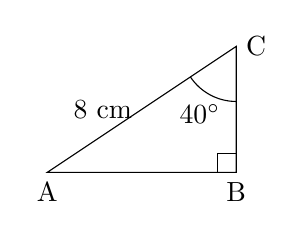
\begin{tikzpicture}[scale=0.8]
% Triangle coordinates
\coordinate (A) at (0,0);
\coordinate (B) at (3,0);
\coordinate (C) at (3,2);

% Draw triangle
\draw (A) -- (B) -- (C) -- cycle;

% Right angle at B
\draw (3,0) rectangle +(-0.3,0.3);

% Labels for vertices
\node[below] at (A) {A};
\node[below] at (B) {B};
\node[right]  at (C) {C};

% Side length AC
\node[left] at ($(A)!0.5!(C)$) {$8\text{ cm}$};

% Angle at C (theta = 40°)
\pic [draw, -, "$40^\circ$", angle eccentricity=1.4, angle radius=0.7cm]
{angle = A--C--B};
\end{tikzpicture}

\vspace{0.3em}
Find the length of BC. \ashow{$8\cos 40^\circ \approx 6.13~\text{cm}$}

% -------- Question 2: Trig - Find the angle --------

\textbf{2.}
\vspace{0.3em}
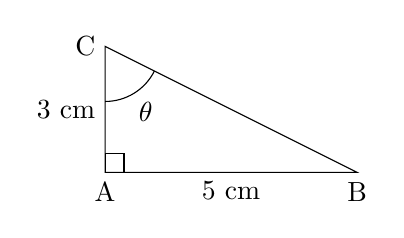
\begin{tikzpicture}[scale=0.8]
% Coordinates
\coordinate (A) at (0,0);
\coordinate (B) at (4,0);
\coordinate (C) at (0,2);

% Triangle
\draw (A) -- (B) -- (C) -- cycle;

% Right angle at A
\draw (A) rectangle +(0.3,0.3);

% Vertex labels
\node[below] at (A) {A};
\node[below] at (B) {B};
\node[left]  at (C) {C};

% Side labels
\node[below] at ($(A)!0.5!(B)$) {$5\text{ cm}$};  % AB
\node[left]  at ($(A)!0.5!(C)$) {$3\text{ cm}$};  % AC

% Angle at C (angle ACB)
\pic [draw, -, "$\theta$", angle eccentricity=1.4, angle radius=0.7cm]
{angle = A--C--B};

\end{tikzpicture}

\vspace{0.3em}
Find $\theta$ \ashow{$\approx 59.0^\circ$}

\end{column}

% ---------------- RIGHT COLUMN ----------------
\begin{column}{0.48\textwidth}

\textbf{3.}

\begin{columns}[T,onlytextwidth]
  \begin{column}{0.55\textwidth}
    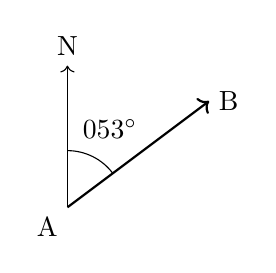
\begin{tikzpicture}[scale=0.9]
      % Points
      \coordinate (A) at (0,0);
      \coordinate (B) at (2,1.5);

      % Bearing line B from A
      \draw[->, thick] (A) -- (B);

      % North at A
      \draw[->] (A) -- +(0,2) node[above] {N};

      % Angle arc at A: 053° clockwise from North
      \draw (0,0) ++(0,0.8) arc[start angle=90, end angle=37, radius=0.8];
      \node at (0.6,1.1) {$053^\circ$};

      % Labels
      \node[below left] at (A) {A};
      \node[right]      at (B) {B};
    \end{tikzpicture}
  \end{column}
  \begin{column}{0.45\textwidth}
    The bearing of \textbf{B from A} is \(\,053^\circ\).\\[0.3em]
    What is the bearing of \textbf{A from B}\,\ashowq{$233^\circ$}
  \end{column}
\end{columns}


% -------- Question 4: Directions at right angles --------
\textbf{4.}

\begin{columns}[T,onlytextwidth]
  \begin{column}{0.55\textwidth}
    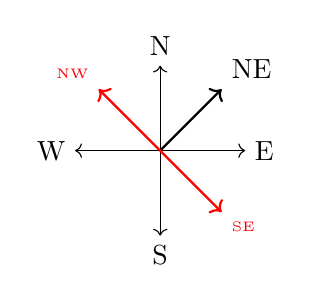
\begin{tikzpicture}[scale=0.6]
      % Compass rose
      \draw[->] (0,0) -- (0,1.8) node[above] {N};
      \draw[->] (0,0) -- (1.8,0) node[right] {E};
      \draw[->] (0,0) -- (0,-1.8) node[below] {S};
      \draw[->] (0,0) -- (-1.8,0) node[left] {W};

      % NE arrow
      \draw[->, thick] (0,0) -- (1.3,1.3) node[above right] {NE};

      % Answer: NW and SE
      \draw[->, ans] (0,0) -- (-1.3,1.3) node[anslab, above left] {NW};
      \draw[->, ans] (0,0) -- (1.3,-1.3) node[anslab, below right] {SE};
    \end{tikzpicture}
  \end{column}
  \begin{column}{0.45\textwidth}
    Which directions are at right angles to \textbf{Northeast}\,?
  \end{column}
\end{columns}

\end{column}
\end{columns}

\end{frame}

% ------------------------------------------------------------------
% Worked Solution: Starter 1, Question 1
% ------------------------------------------------------------------
\begin{frame}{Worked Solution: Retrieve and Connect 1, Question 1}
\hypertarget{work-st1}{}

\textbf{Question:} In right-angled triangle \(ABC\), the right angle is at \(B\), \(AC = 8\text{ cm}\), and \(\angle ACB = 40^\circ\). Find the length of \(BC\).

\textbf{Worked Solution:}

Relative to the \(40^\circ\) angle at \(C\):
\begin{itemize}
\item The \textbf{hypotenuse} is \(AC = 8\text{ cm}\).
\item The side \(BC\) is \textbf{adjacent} to the angle.
\item The side \(AB\) is \textbf{opposite} the angle.
\end{itemize}

Since we know the hypotenuse and want the adjacent side, we use the cosine ratio:

\[
\cos 40^\circ = \frac{\text{adjacent}}{\text{hypotenuse}} = \frac{BC}{AC} = \frac{BC}{8}
\]

Rearranging gives:

\[
BC = 8\cos 40^\circ
\]

Using a calculator:

\[
BC \approx 8 \times 0.7660 \approx 6.13\text{ cm}
\]

\[
\boxed{BC \approx 6.13\text{ cm}}
\]

\end{frame}

% ------------------------------------------------------------------
% Worked Solution: Starter 1, Question 2
% ------------------------------------------------------------------
\begin{frame}{Worked Solution: Retrieve and Connect 1, Question 2}

\textbf{Question:} In right-angled triangle \(ABC\), the right angle is at \(A\), \(AB = 5\text{ cm}\), and \(AC = 3\text{ cm}\). Find the angle \(\theta\) at \(C\).

\textbf{Worked Solution:}

Relative to angle \(\theta\) at \(C\):
\begin{itemize}
\item The side \(AB = 5\text{ cm}\) is \textbf{opposite} the angle.
\item The side \(AC = 3\text{ cm}\) is \textbf{adjacent} to the angle.
\end{itemize}

Since we know the opposite and adjacent sides, we use the tangent ratio:

\[
\tan\theta = \frac{\text{opposite}}{\text{adjacent}} = \frac{AB}{AC} = \frac{5}{3}
\]

So:

\[
\theta = \tan^{-1}\left(\frac{5}{3}\right)
\]

Using a calculator:

\[
\theta \approx \tan^{-1}(1.6667) \approx 59.0^\circ
\]

\[
\boxed{\theta \approx 59.0^\circ}
\]

\end{frame}

% ------------------------------------------------------------------
% Worked Solution: Starter 1, Question 3
% ------------------------------------------------------------------
\begin{frame}{Worked Solution: Retrieve and Connect 1, Question 3}

\textbf{Question:} The bearing of \(B\) from \(A\) is \(053^\circ\). What is the bearing of \(A\) from \(B\)?

\textbf{Worked Solution:}

Bearings are measured clockwise from North. The bearing of \(A\) from \(B\) is the \textbf{back bearing}; reverse directions differ by \(180^\circ\).

Since \(053^\circ < 180^\circ\), we add \(180^\circ\):

\[
053^\circ + 180^\circ = 233^\circ
\]

\[
\boxed{\text{The bearing of } A \text{ from } B \text{ is } 233^\circ}
\]

\end{frame}

% ------------------------------------------------------------------
% Worked Solution: Starter 1, Question 4
% ------------------------------------------------------------------
\begin{frame}{Worked Solution: Retrieve and Connect 1, Question 4}

\textbf{Question:} Which directions are at right angles to \textbf{Northeast}?

\textbf{Worked Solution:}

Northeast is halfway between North and East, so its bearing is:

\[
045^\circ
\]

Directions at right angles are \(90^\circ\) away:

\[
045^\circ + 90^\circ = 135^\circ
\]

A bearing of \(135^\circ\) is \textbf{Southeast}.

\[
045^\circ - 90^\circ = -45^\circ
\]

Since bearings are conventionally measured between \(0^\circ\) and \(360^\circ\):

\[
-45^\circ + 360^\circ = 315^\circ
\]

A bearing of \(315^\circ\) is \textbf{Northwest}.

\[
\boxed{\text{Northwest and Southeast}}
\]

\end{frame}

\end{document}